\documentclass[mathserif,spanish]{beamer}

\mode<presentation>{
\usetheme{Warsaw}
\setbeamertemplate{footline}[page number]
}

\usepackage{graphicx}
\usepackage{booktabs} 
\usefonttheme{professionalfonts}
\usepackage[justification=centering]{caption}
\usepackage{ragged2e}
\justifying
\usepackage[utf8]{inputenc} 
\usepackage[spanish]{babel}

\title[Lab 2]{Resultados del laboratorio 2}
\subtitle{Grupo B}
\author[E.Castro \and D.Chavarría \and E.Segura]{E.Castro \and D.Chavarría \and E.Segura}
\institute[TEC]{
Instituto Tecnológico de Costa Rica\\
Escuela de Ingeniería Electrónica \\
Laboratorio de Control Automático}
\date{\today}

\begin{document}

\begin{frame}[plain]
\begin{center}

\includegraphics [height=3cm,width=6cm]{Figures/TEC.png}
\end{center}
\titlepage
\end{frame}

\begin{frame}{Contenidos}
\tableofcontents
\end{frame}

%------------------------------------------------
\section{Objetivo}

\begin{frame}{Objetivo}
\begin{itemize}
\item Identificar experimentalmente la planta PADP.
\item Diseñar y evaluar controladores PID, REI y I-PD.
\item Comparar desempeño en simulación y experimento.
\item Validar cumplimiento de especificaciones:
\begin{itemize}
\item $t_s \leq 5$ s
\item $M_p \leq 3\%$
\end{itemize}
\end{itemize}
\end{frame}

%------------------------------------------------
\section{Resumen}

\begin{frame}{Resumen}
\begin{itemize}
\item Obtención de datos experimentales de la planta.
\item Construcción de modelo promedio representativo.
\item Diseño de múltiples estrategias de control.
\item Evaluación comparativa entre simulación y resultados reales.
\end{itemize}
\end{frame}

%------------------------------------------------
\section{Metodología}

\subsection{Obtención de datos}

\begin{frame}{Obtención de datos}
\begin{itemize}
\item Se realizaron 3 tomas experimentales.
\item Medición de respuesta al escalón.
\item Extracción de parámetros dinámicos.
\end{itemize}
\end{frame}

\subsection{Estadística}

\begin{frame}{Estadística de la planta}
\begin{itemize}
\item Cálculo de parámetros promedio:
\begin{itemize}
\item Frecuencia natural $\omega_n$
\item Factor de amortiguamiento $\zeta$
\end{itemize}
\item Reducción de variabilidad mediante promediado.
\end{itemize}
\end{frame}

\subsection{Descarte}

\begin{frame}{Descarte de la toma 3}
\begin{itemize}
\item Alta desviación respecto a otras muestras.
\item Incremento del coeficiente de variación (CV).
\item Se descarta para mejorar precisión del modelo.
\end{itemize}
\end{frame}

\section{Controladores}

\begin{frame}{Controladores utilizados}
\begin{itemize}
\item PID (Sintonización clásica / SISOtool)
\item REI (LQR con acción integral)
\item I-PD (Ubicación de polos)
\item Comparación de desempeño entre técnicas
\end{itemize}
\end{frame}

%------------------------------------------------
\subsection{Resultados PID}

\begin{frame}{Metodología PID}
\begin{itemize}
\item Diseño mediante ajuste de ganancias.
\item Evaluación en simulación y sistema real.
\end{itemize}
\end{frame}

\begin{frame}{Simulación PID}
\centering
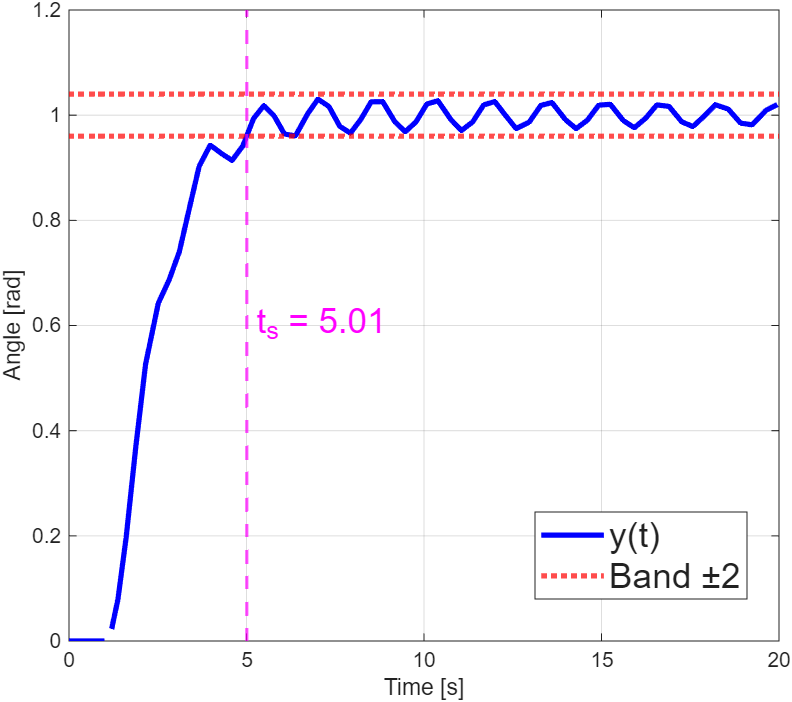
\includegraphics[width=0.8\linewidth]{Figures/simulation_PID.png}
\end{frame}

\begin{frame}{Experimental PID}
\centering
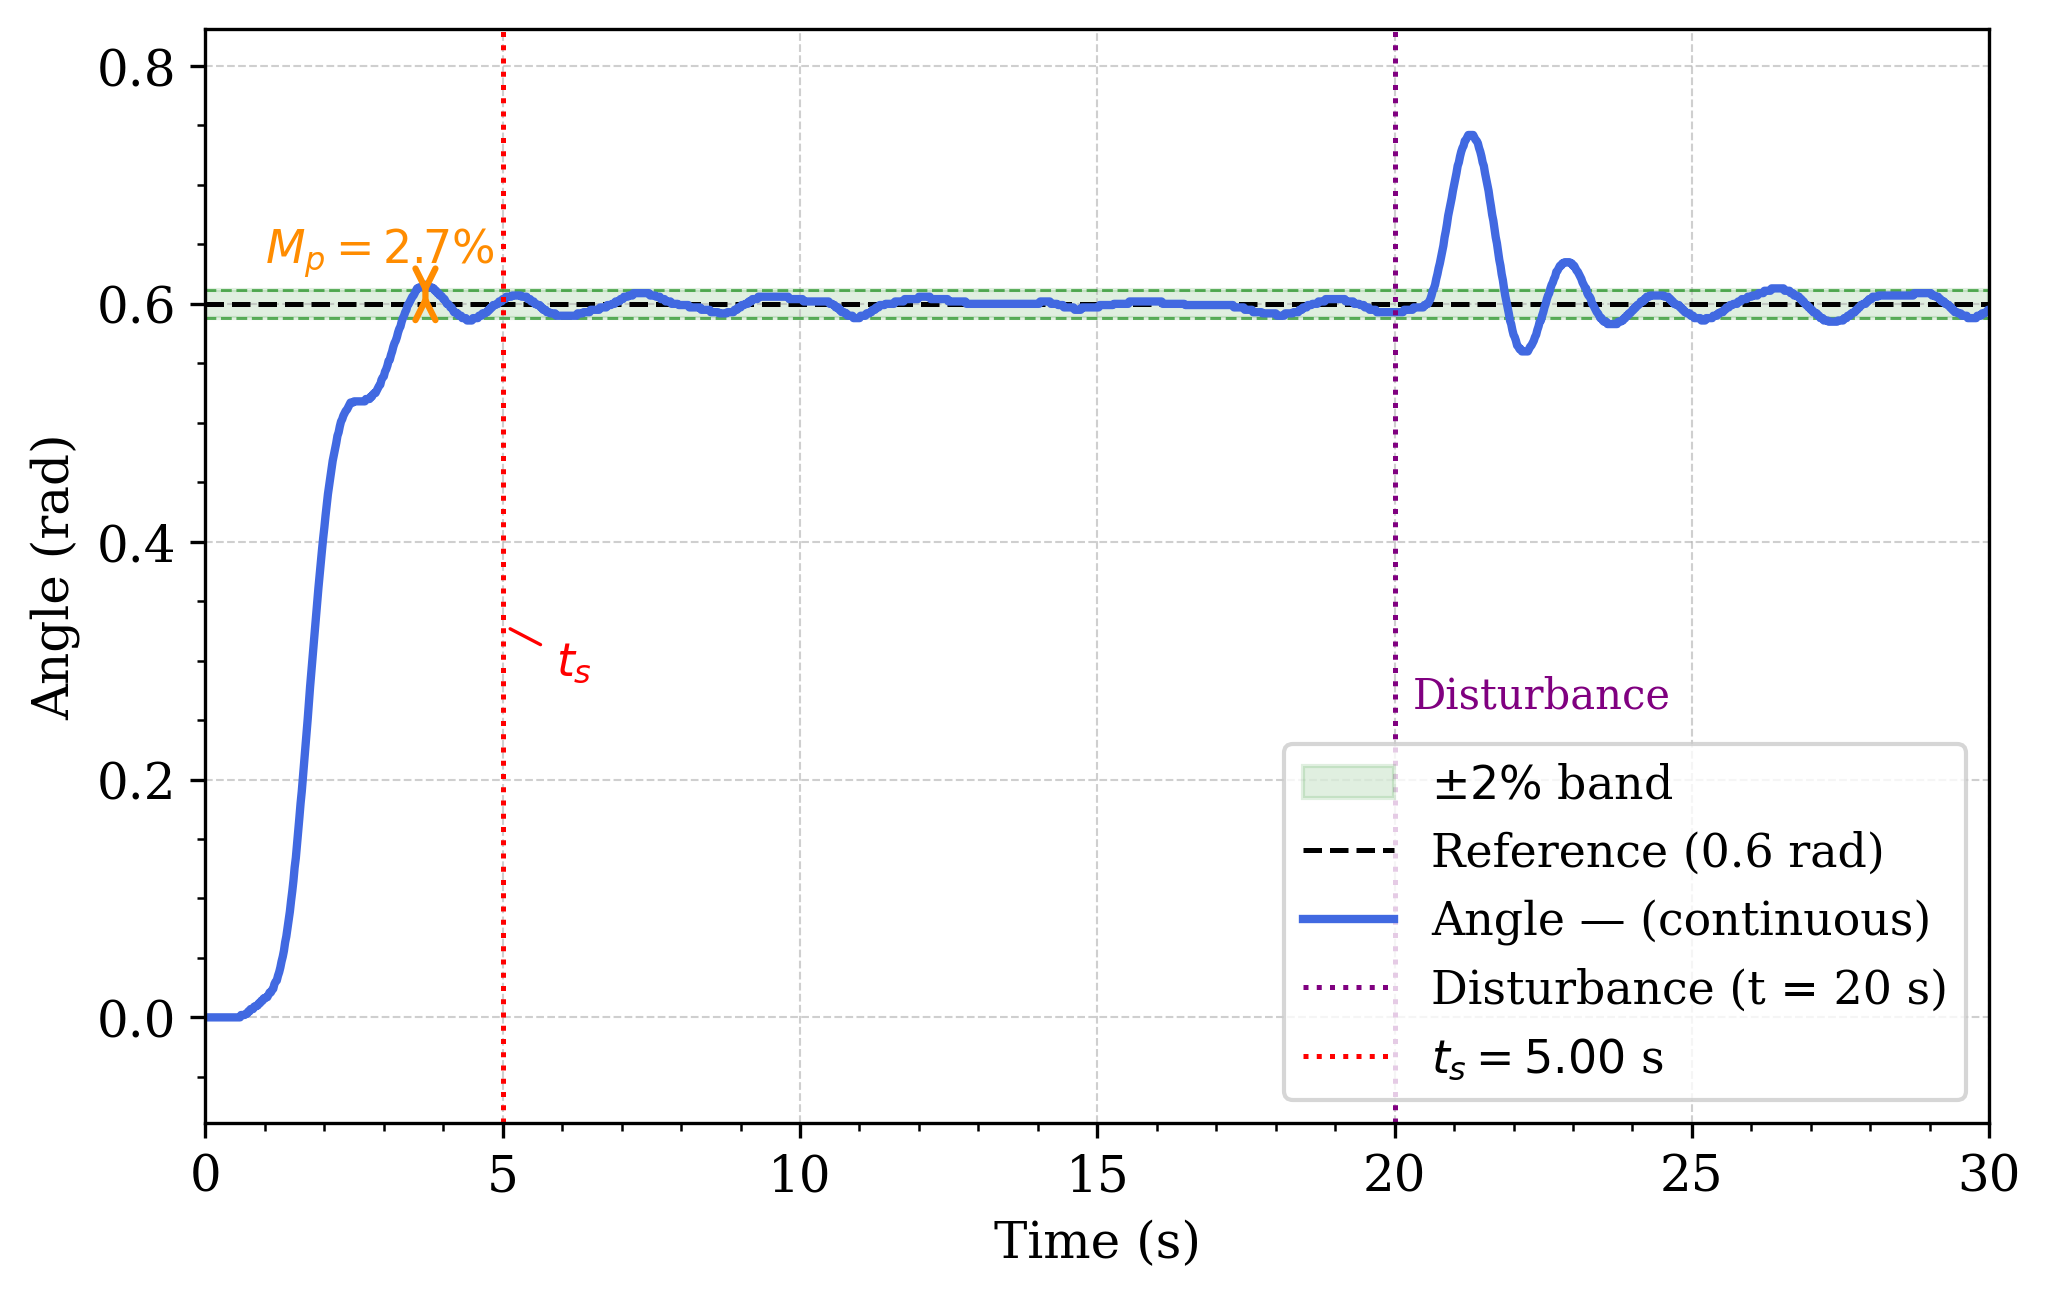
\includegraphics[width=0.8\linewidth]{Figures/experimental_pid.png}
\end{frame}

\begin{frame}{Comparativa PID}
\centering
\begin{tabular}{lccc}
\toprule
Condición & $t_s$ & $M_p$ & Cumple \\
\midrule
Simulación & - & - & - \\
Experimental & - & - & - \\
\bottomrule
\end{tabular}
\end{frame}

%------------------------------------------------
\subsection{Resultados REI}

\begin{frame}{Metodología REI}
\begin{itemize}
\item Diseño mediante LQR con acción integral.
\item Minimización de error estacionario.
\end{itemize}
\end{frame}

\begin{frame}{Simulación REI}
\centering
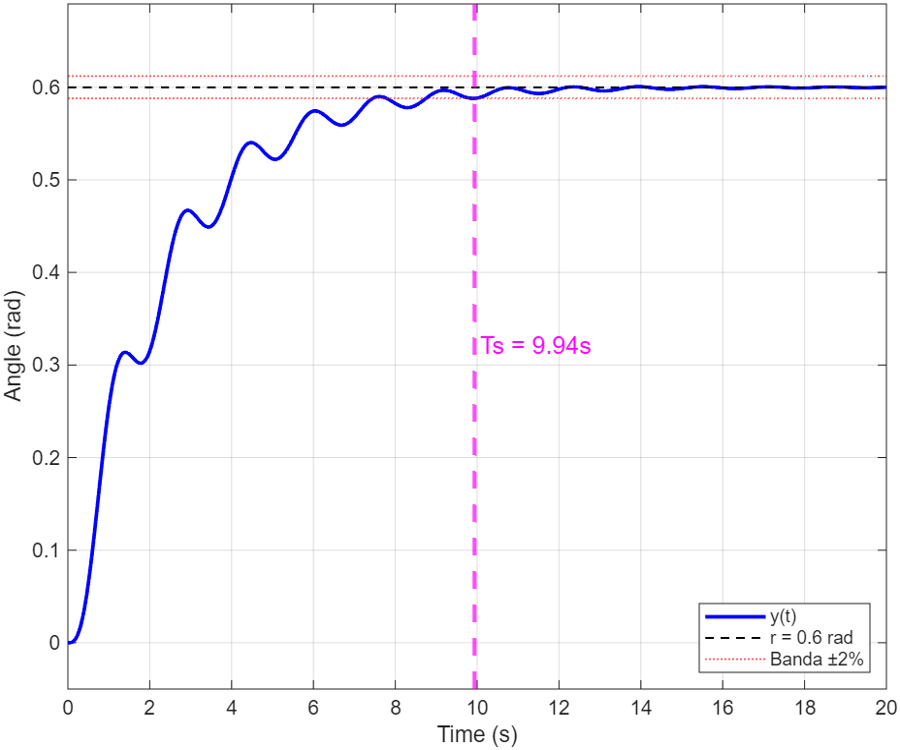
\includegraphics[width=0.8\linewidth]{Figures/simulation_rei.png}
\end{frame}

\begin{frame}{Experimental REI}
\centering
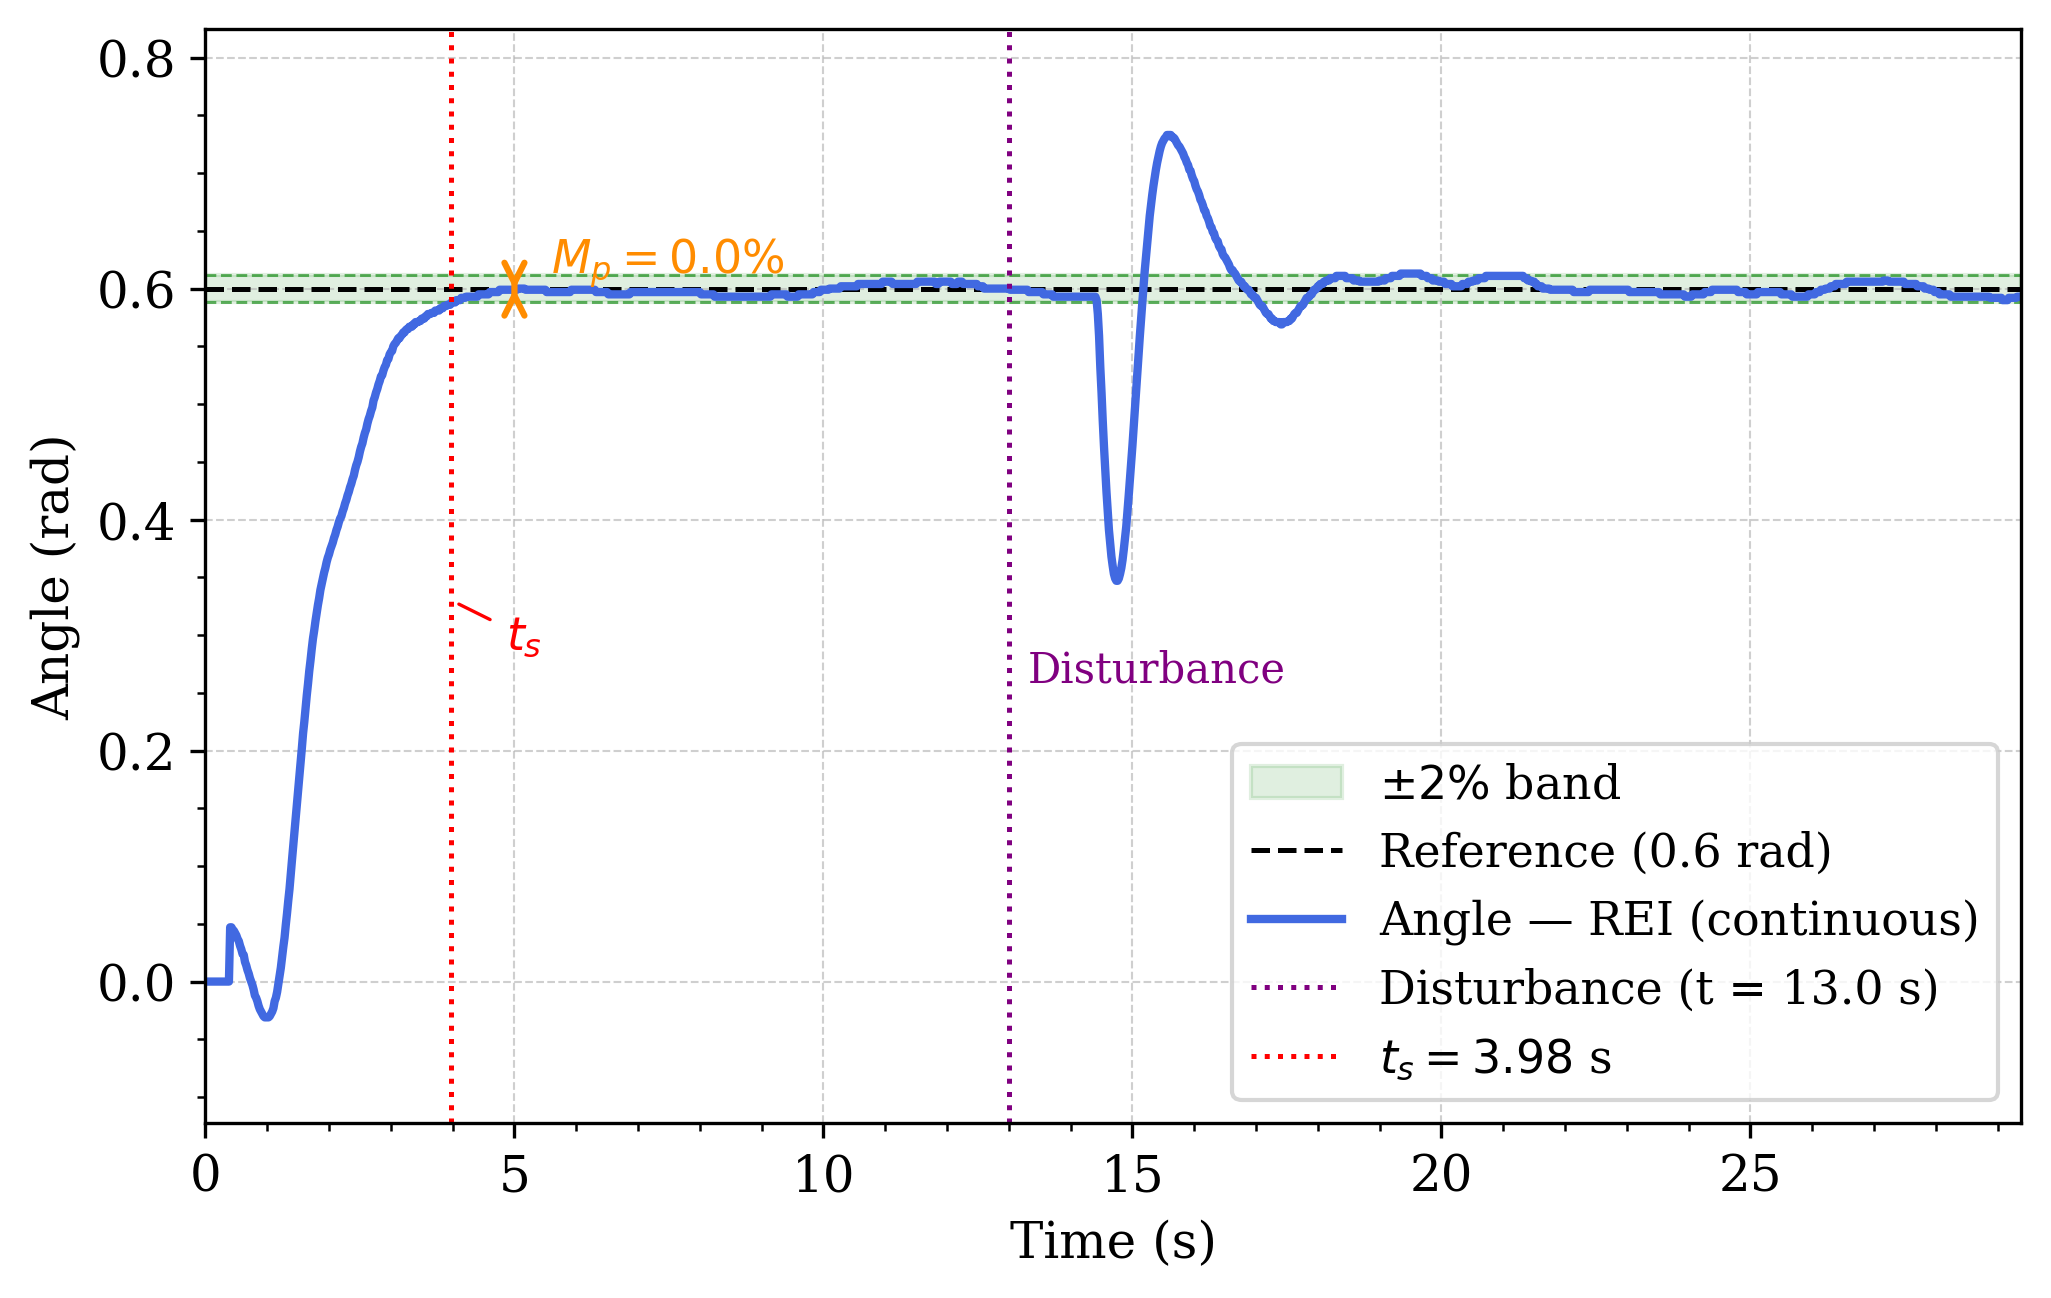
\includegraphics[width=0.8\linewidth]{Figures/experimental_rei.png}
\end{frame}

\begin{frame}{Comparativa REI}
\centering
\begin{tabular}{lccc}
\toprule
Condición & $t_s$ & $M_p$ & Cumple \\
\midrule
Simulación & 9.94 s & 0.12\% & No \\
Experimental & 3.98 s & 0\% & Sí \\
\bottomrule
\end{tabular}
\end{frame}

%------------------------------------------------
\subsection{Resultados I-PD}

\begin{frame}{Metodología I-PD}
\begin{itemize}
\item Diseño por ubicación de polos.
\item Separación de acción proporcional y derivativa.
\end{itemize}
\end{frame}

\begin{frame}{Simulación I-PD}
\centering
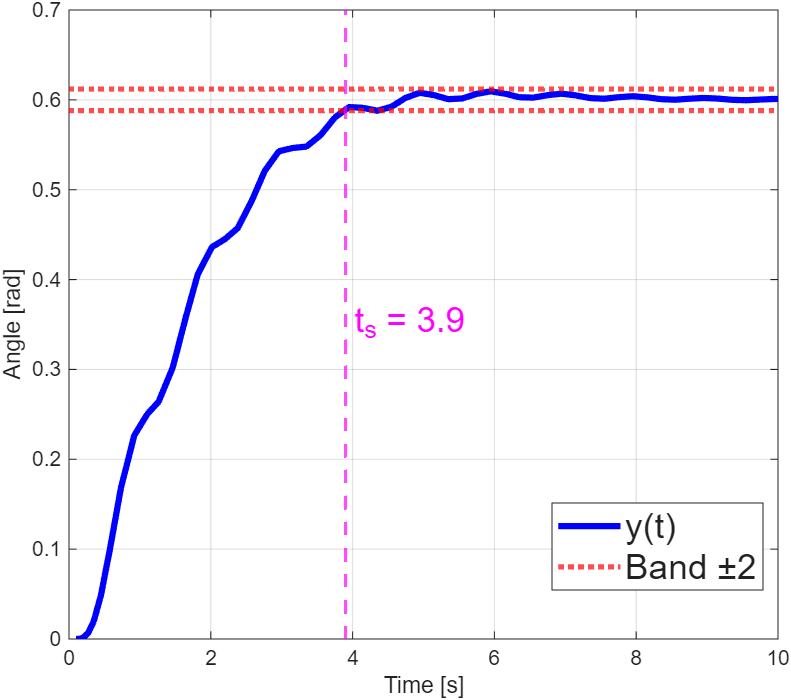
\includegraphics[width=0.8\linewidth]{Figures/simulation_IPD.png}
\end{frame}

\begin{frame}{Experimental I-PD}
\centering
\includegraphics[width=0.8\linewidth]{Figures/ipd_exp.png}
\end{frame}

\begin{frame}{Comparativa I-PD}
\centering

\begin{tabular}{lccc}
\toprule
Condición & $t_s$ & $M_p$ & Cumple \\
\midrule
Simulación & - & - & - \\
Experimental & - & - & - \\
\bottomrule
\end{tabular}
\end{frame}

%------------------------------------------------
\subsection{Discusión}

\begin{frame}{Discusión}
\begin{itemize}
\item Comparación entre controladores.
\item Evaluación del mejor desempeño.
\item Diferencias entre simulación y experimento.
\item Influencia del modelo de la planta.
\end{itemize}
\end{frame}

\begin{frame}{Mejor controlador}
\begin{itemize}
\item Selección basada en:
\begin{itemize}
\item Tiempo de establecimiento
\item Sobreimpulso
\item Error estacionario
\end{itemize}
\item Justificación técnica del mejor método.
\end{itemize}
\end{frame}

%------------------------------------------------
\section{Conclusiones}

\begin{frame}{Conclusiones}
\begin{itemize}
\item Cada controlador presenta ventajas específicas.
\item El REI destaca en error estacionario nulo.
\item El PID ofrece simplicidad de implementación.
\item Se logró cumplir parcialmente las especificaciones.
\end{itemize}
\end{frame}

%------------------------------------------------
\subsection{Recomendaciones}

\begin{frame}{Recomendaciones}
\begin{itemize}
\item Utilizar más sets de datos para reducir el CV.
\item Descartar muestras atípicas.
\item Ajustar parámetros teóricos de forma conservadora.
\item Mejorar la identificación experimental de la planta.
\end{itemize}
\end{frame}

%------------------------------------------------
\section{Bibliografía}

\begin{frame}{Bibliografía}
\footnotesize
\begin{thebibliography}{9}
\bibitem{ogata} Ogata, Modern Control Engineering.
\bibitem{ljung} Ljung, System Identification.
\bibitem{astrom} Åström, PID Control.
\end{thebibliography}
\end{frame}

\end{document}